\begin{figure*}[t]
\centering
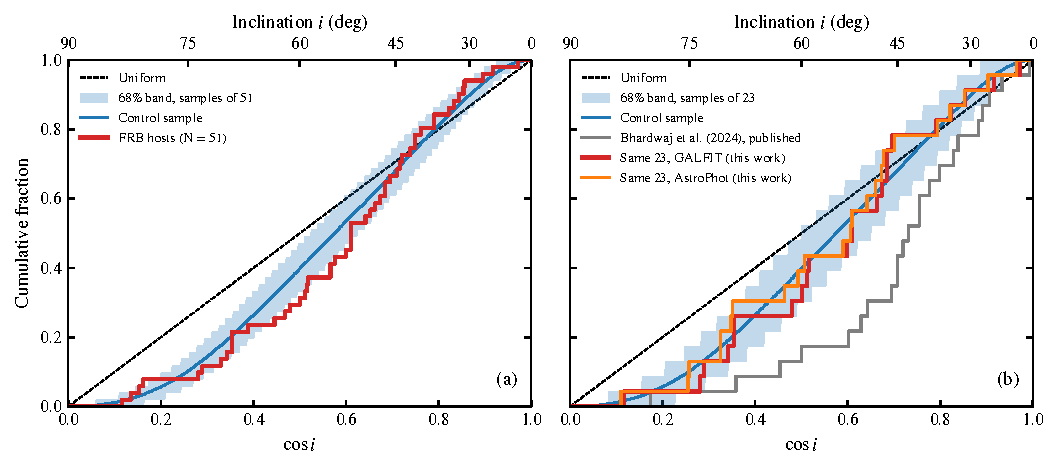
\includegraphics[width=\textwidth]{fig1_cdf.pdf}
\caption{CDFs of $\cos i$. (a) The 51 FRB hosts (red) and the control sample
(blue), with the 68\% bound of 10{,}000 random samples of 51 control galaxies
(shaded). (b) The 23 hosts of \citet{Bhardwaj2024}, using their published
inclinations (grey), our \textsc{galfit} remeasurement (red) and an independent
\textsc{AstroPhot} remeasurement of the same images (orange; RMS difference
between the two codes $3.0^\circ$), with the 68\% bound for samples of 23.
The dashed line shows a uniform distribution.}
\label{fig:cdf}
\end{figure*}

\begin{figure}[t]
\centering
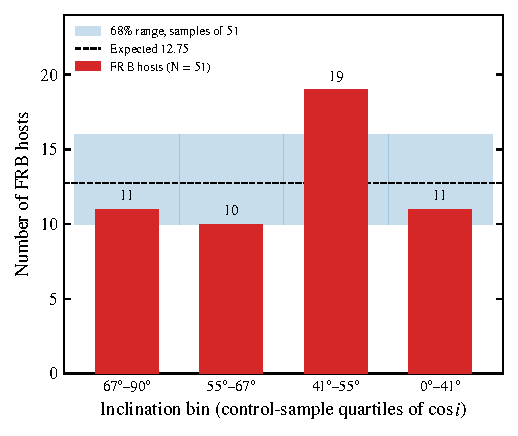
\includegraphics[width=\columnwidth]{fig2_bins.pdf}
\caption{Number of FRB hosts in each of four inclination bins, defined by the
quartiles of the control sample's $\cos i$ distribution; the bin ranges are
marked on the horizontal axis. The dashed line marks the expected 12.75 hosts
per bin, and the shaded band the 68\% range from random samples of 51 control
galaxies.}
\label{fig:bins}
\end{figure}
